% !TeX spellcheck = cs_CZ
%{\tikzset{external/prefix={tikz/FYZII/}}
% \tikzset{external/figure name/.add={ch30_}{}}
%---------------------------------------------------------------------------------------------------
% file fey2ch30.tex
%---------------------------------------------------------------------------------------------------
%=========================== Kapitola Vnitřní geometrie krystalů ===================================
\chapter{Vnitřní geometrie krystalů}\label{fyz:IIchapXXX}
\minitoc
  \section{Vnitřní geometrie krystalů}\label{fyz:IIchapXXXsecI}
    Studium základních zákonů elektřiny a magnetizmu jsme ukončili a nyní se budeme věnovat studiu 
    elektromagnetických vlastností látky. Začneme popisem pevných látek, tj. krystalů. Když se 
    atomy v látce příliš nepohybují, zůstávají seskupeny jeden u druhého v konfiguraci s nejnižší 
    možnou energií. Jestliže se atomy v jednom místě uspořádají tak, aby měly malou energii, je 
    pravděpodobné, že se na nějakém jiném místě uspořádají stejně. To je důvod, proč se v pevných 
    látkách opakují stejné konfigurace atomů.

    Jinými slovy, podmínky v krystalu jsou následující: Okolí každého atomu v krystalu je určitým 
    způsobem uspořádáno a podíváme-li se na atom stejného druhu na jiném, vzdálenějším místě, 
    zjistíte, že jeho okolí je přesně stejné. A vybereme-li si jiný atom, vzdálený o tutéž 
    vzdálenost, ještě dále, zjistíme, že podmínky jsou opět tytéž. Uspořádání se opakuje znovu a 
    znovu, samozřejmě, ve všech třech rozměrech.

    \begin{figure}[ht!]  %\ref{fyz_fig733}
      \centering
      \begin{tabular}{cc}
        \subfloat[ ]{\label{fyz_fig733a}
          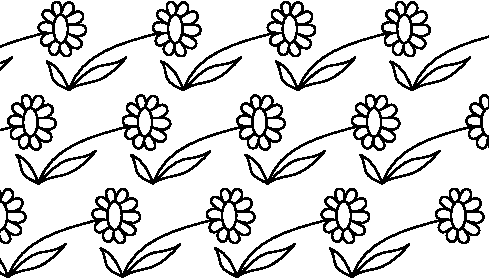
\includegraphics[width=0.45\linewidth]{fyz_fig733a.pdf}}               &
        \subfloat[ ]{\label{fyz_fig733b}
          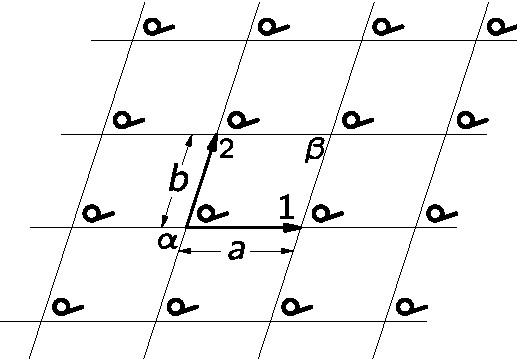
\includegraphics[width=0.45\linewidth]{fyz_fig733b.pdf}} 
      \end{tabular}
      \caption{Opakující se vzorek ve dvou rozměrech 
               (\cite[s.~748]{Feynman02})}
      \label{fyz_fig733}
    \end{figure}
    
    Představme si, že máme navrhnout vzor tapety nebo látky, nebo nějaký jiný geometrický vzor na 
    rovinné ploše, přičemž se předpokládá, že navrhneme nějaký prvek, který se bude opakovat po tak 
    velké ploše, jak jen budeme chtít. Je to dvojrozměrná analogie problému, který se v krystalu 
    řeší ve třech rozměrech. Například obr. \ref{fyz_fig733a} představuje běžný druh tapetového 
    vzoru. Je tu jediný prvek, který se ve vzoru neustále opakuje. Geometrická charakteristika 
    tapetového dezénu, bereme-li v úvahu jen jeho periodické vlastnosti a nezajímáme se o geometrii 
    nebo uměleckou hodnotu samotného květu, je znázorněna na obr. \ref{fyz_fig733b}. Když začneme v 
    libovolném bodě, můžeme najít \emph{analogický} bod posunem o vzdálenost \(a\) ve směru šipky 
    \(1\). Analogický bod můžeme dostat i tehdy, posuneme-li se o vzdálenost \(b\) ve směru druhé 
    šipky. Existují, samozřejmě, i jiné směry. Můžeme například jít přímo z bodu \(\alpha\) do 
    \(\beta\)  dostat se do analogické polohy, jenže takový krok může být považován za postupnou 
    kombinaci kroků podél směru \(1\) a pak podél směru \(2\). Jedna ze základních vlastností vzoru 
    může být popsána dvěma nejkratšími kroky ke stejným sousedním polohám.
    
    \begin{figure}[ht!]
      \centering
      \begin{tabular}{cc}
        \subfloat[ ]{\label{fyz_fig734}
          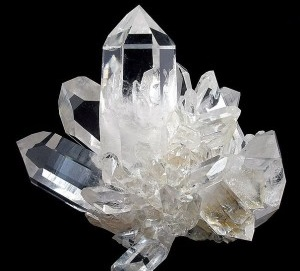
\includegraphics[width=0.45\linewidth]{fyz_fig734_1.jpg}}              &
        \subfloat[ ]{\label{fyz_fig735}
          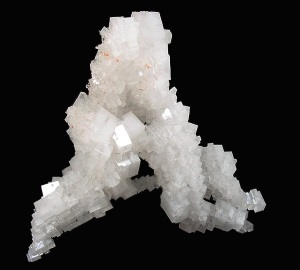
\includegraphics[width=0.45\linewidth]{fyz_fig735_1.jpg}}              \\
        \subfloat[ ]{\label{fyz_fig736}
          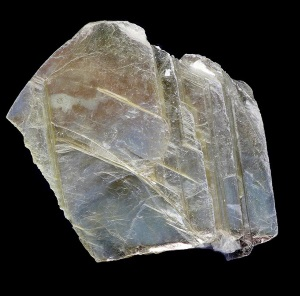
\includegraphics[width=0.45\linewidth]{fyz_fig736_1.jpg}}
      \end{tabular}
      \caption{Přírodní krystaly: a) křemen b) chlorid sodný, c) slída
               (\cite[s.~545]{Feynman02})}
    \end{figure}

    Stejnými polohami myslíme, že kdybychom stáli v některé z těchto poloh a podívali bychom se 
    kolem, viděli bychom přesně totéž, jako kdybychom stáli v některé jiné poloze. To je základní 
    vlastnost krystalu. Jediný rozdíl jev tom, že krystal představuje trojrozměrné uspořádání místo 
    dvojrozměrného a, přirozeně, že místo květů představuje každý prvek mřížky určité uspořádání 
    atomů do nějaké konfigurace (například šest atomů vodíku a dva atomy uhlíku). Uspořádání atomů 
    v krystalu lze zjistit experimentálně pomocí rentgenové difrakce. 
    
    Vnitřní stavba krystalu se projevuje více způsoby. Za prvé, síla, která váže atomy navzájem, je 
    obvykle silnější v jednom směru než ve druhém. To znamená, že v krystalu existují plochy, podél 
    nichž je možné krystal snáze rozštěpit. Nazývají se \emph{štěpné} plochy. Rozbijeme-li krystal 
    čepelí nože, rozštěpí se většinou podél této plochy. Za druhé, vnitřní struktura je často 
    viditelná na povrchu díky způsobu, jakým krystal vznikl. Představme si, že se krystal vytváří 
    usazováním z roztoku. Atomy se v roztoku volně vznášejí až se nakonec, když najdou polohy s 
    nejnižší energií, usadí. (Je to, jako kdyby tapeta vznikala tak, že kvítky poletují sem a tam, 
    až se jeden náhodně dostane na určité místo a zůstane tam přilepen. Stejně je to s dalšími, až 
    se postupně vytváří celý vzor.) Chápeme, že v některých směrech roste krystal rychleji než v 
    jiných, a tím získává při růstu nějaký geometrický tvar. Díky tomuto jevu povrch mnoha krystalů 
    něco odráží z vlastností vnitřního uspořádání atomů,
    
    Tak například \ref{fyz_fig734} je znázorněn typický tvar krystalu křemene, jehož vnitřní 
    struktura je hexagonální. Všimneme-li si blíže celého krystalu, zjistíme, že zvenku to není 
    dokonalý šestiboký hranol, neboť stěny nejsou stejné dlouhé - ve skutečnosti bývají délkové 
    rozdíly dost velké. Ale z jednoho hlediska jde o velmi pravidelný šestiúhelník, \emph{úhly} 
    mezi stěnami mají přesně \SI{120}{\deg}. Je zřejmé, že velikosti té či oné hrany souvisí s 
    náhodnými procesy růstu, ale \emph{úhly} reprezentují vnitřní symetrii. Proto každý krystal 
    křemene má jiný tvar, ačkoliv úhly mezi jednotlivými stěnami jsou vždy tytéž. 
    
    Vnitřní symetrie krystalu chloridu sodného je také zřejmá z jeho vnějšího tvaru. Na obr. 
    \ref{fyz_fig735} je znázorněn typický tvar krystalu soli. Opět krystal není dokonalou krychlí, 
    ale stěny svírají přesně pravý úhel. 
    
    Komplikovanějším krystalem je slída, jejíž tvar je na obr. \ref{fyz_fig736}. Je to krystal s 
    velkým stupněm \emph{anizotropie}. Je to vidět i z toho, že je velmi těžké slídu v jednom směru 
    (na obrázku horizontálně), ale v jiném směru (vertikálně) ji lze štěpit velmi snadno. Tato 
    vlastnost se využívala k získávání velmi pevných tenkých vrstev. Slída a křemen jsou dva 
    příklady přírodních nerostů obsahujících oxid křemičitý. Dalším takovým příkladem je azbest, 
    který má tu vlastnost, že je snadno štěpitelný ve dvou směrech, ale ve třetím ne. Je vytvořen z 
    velmi silných \emph{lineárních} vláken. 
    
  \section{Chemické vazby v krystalech}\label{fyz:IIchapXXXsecII}
    Mechanické vlastnosti krystalů zřejmě závisejí na druhu chemických vazeb mezi atomy. Zarážející 
    rozdíly v pevnosti podél různých směrů ve slídě závisejí na druhu meziatomových vazeb v různých 
    směrech. V chemii jsme se učili o různých druzích chemických vazeb. Za prvé, jsou to 
    \emph{iontové vazby} o nichž jsme už hovořili v souvislosti s chloridem sodným. Zhruba řečeno, 
    atomy vodíku ztratí jeden elektron a stávají se kladnými ionty. Atomy chloru získají jeden 
    elektron a stávají se zápornými ionty. Kladné a záporné ionty jsou uspořádány do trojrozměrné 
    šachovnice a drží se navzájem elektrickými silami. 
    
    \begin{figure}[ht!] %\ref{fyz_fig737}
      \centering
      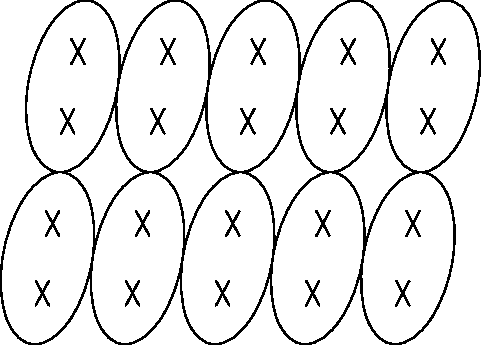
\includegraphics[width=0.5\linewidth]{fyz_fig737.pdf}
      \caption{Mřížka molekulového krystalu 
               (\cite[s.~546]{Feynman02})}
      \label{fyz_fig737}
    \end{figure}
    
    \emph{Kovalentní vazba}, v níž mají dva atomu společné elektronu, se vyskytuje častěji a 
    obvykle je velmi silná. 
    
    Například v diamantu jsou atomy uhlíku vázány kovalentně s nejbližšími sousedními atomy ve 
    všech čtyřech směrech, a proto je krystal skutečně velmi pevný. Kovalentní vazba je i mezi 
    křemíkem a kyslíkem v krystalu křemene, ale ve skutečnosti je to vazba jen částečně kovalentní, 
    Elektrony nejsou úplně společné, proto jsou atomy částečně nabité a krystal má v určitém smyslu 
    iontový charakter. Příroda není tak jednoduchá, jak se ji snažíme udělat. Ve skutečnosti 
    existují všechny možné stupně mezi kovalentní a iontovou vazbou.

    Krystal cukru má zase jiný druh vazby. Jsou v něm velké molekuly, jejichž atomy se silně drží 
    navzájem kovalentní vazbou, a proto má molekula tuhou strukturu. Ale jelikož silné vazby jsou 
    zcela nasyceny, zůstává jen relativně slabá přitažlivost mezi jednotlivými oddělenými 
    molekulami V takových \emph{molekulových} krystalech si molekuly zachovávají svou, řekněme, 
    individualitu a vnitřní uspořádání může být takové, jako vidíme na obr. \ref{fyz_fig737}. 
    Jelikož molekuly nejsou navzájem silně vázány, lze krystal snadno rozbít. Je to něco docela 
    jiného než diamant, který je skutečně jednou velkou molekulou, kterou nelze rozbít, aniž bychom 
    někde narušili kovalentní vazby. Parafín je další příklad molekulového krystalu.
    
    Extrémní příklad molekulového krystalu je pevný argon. Přitažlivost mezi atomy je v něm velmi 
    malá - každý atom je úplně saturovanou jedno atomovou molekulou. Při velmi nízkých teplotách je 
    však tepelný pohyb velmi slabý, proto nepatrné meziatomové síly mohou způsobit, že se atomy 
    uspořádají do pravidelného seskupení podobně jako kuličky při nejtěsnějším uspořádání.
    
    Kovy představují docela jinou třídu látek. Vazba je úplně jiná. Nevážou se sousední atomy, ale 
    vazba se vztahuje na celý krystal. Valenční atomy nepříslušejí jednomu atomu nebo dvojici 
    atomů, ale celému krystalu. Každý atom přispívá svým elektronem do společné „nádrže“ elektronů 
    a kladné ionty „přebývají v moři“ záporných elektronů. Elektronové moře představuje jakési 
    lepidlo, které drží ionty pohromadě.
    
    Jelikož v kovu neexistují žádné speciální vazby v určitém směru, není v jeho stavbě výrazná 
    závislost na směrech. Kovy však stále ještě patří mezi krystalické látky, protože jejich 
    celková energie je nejnižší tehdy, když jsou ionty atomů uspořádány v nějakém určitém seskupení 
    - ačkoliv energie tohoto preferovaného seskupení obvykle není o mnoho nižší než jiné možné 
    energie. V prvním přiblížení jsou atomy mnohých kovů uspořádány jako kuličky při nejtěsnějším 
    seskupení.
    
  \section{Růst krystalů}\label{fyz:IIchapXXXsecIII}
    Pokusme si představit, jak se přirozenou cestou vytvářely krystaly na Zemi. Zemská kůra 
    představuje směs atomů všech druhů. Ty se neustále mísí za pomoci sopečné činnosti, větru a 
    vody. Ale jakýmsi trikem se atomy křemíku postupně navzájem najdou a setkají se s atomy kyslíku 
    a vytvoří křemen. Jeden atom se vždy přidá k dalším a buduje se krystal. Směs přestává být 
    směsí. A kdesi nedaleko se setkávají atomy sodíku a chloru a vytvářejí krystal soli.
    
    Čím to je, že krystal, začne-li se jednou budovat, dovoluje jen určitému druhu atomů, aby se 
    připojoval? Je to tím, že celý systém usiluje o nejnižší možnou energii. Rostoucí krystal 
    přijme nový atom jen tehdy, když spolu s ním bude mít tak nízkou energii, jak je to jen možné. 
    Ale jak krystal ví, že umístěním atomu křemíku nebo kyslíku do určité polohy má zaručenu 
    nejnižší energii? Dělá to metodou pokusů a omylů. V tekutinách jsou všechny atomy v neustálém 
    pohybu. Každý atom naráží na svého souseda přibližně \num{e13}-krát za sekundu. Narazí-li na 
    správné místo v krystalu, kde je nízká energie, je menší pravděpodobnost, že se odrazí zpět. 
    Postupným zkoušením po dobu milionů let, při \num{e13} pokusech za sekundu, atomy postupně 
    budují krystal v místech, kde dosáhnou nejnižší energii. Nakonec tak narostou velké krystaly.
    
  \section{Krystalové mřížky}\label{fyz:IIchapXXXsecIV}
    Uspořádání atomů v krystalu - \textbf{krystalová mřížka} - může mít různé geometrické tvary. 
    Nejdříve popíšeme nejjednodušší mřížky, které jsou charakteristické pro většinu kovů a pro 
    inertní plyny v pevném skupenství. Jsou to krychlové mřížky, které se mohou vyskytovat ve dvou 
    tvarech: \emph{Prostorově centrovaná} (obr. \ref{fyz_fig738a}) a \emph{plošně centrovaná} 
    krychlová mřížka (obr. \ref{fyz_fig738b}). Nákresy samozřejmě znázorňují jen jednu krychli 
    mřížky. Musíme si představit, že vzor se opakuje do nekonečna ve třech rozměrech. Aby byl 
    obrázek názornější, jsou nakresleny jen „středy“ atomů. Ve skutečném krystalu jsou atomy téměř 
    jako koule, které jsou ve vzájemném kontaktu. Tmavé a světlé kuličky na obrázku mohou obecně 
    představovat buď různé, nebo stejné druhy atomů. Například železo má při nízkých teplotách 
    prostorově centrovanou krychlovou mřížku, ale při vysokých teplotách má plošně centrovanou 
    krychlovou mřížku. Fyzikální vlastnosti těchto dvou druhů krystalů jsou docela odlišné.
    
    \begin{figure}[ht!]   %\ref{fyz_fig738}
      \centering
      \begin{tabular}{cc}
        \subfloat[ ]{\label{fyz_fig738a}
          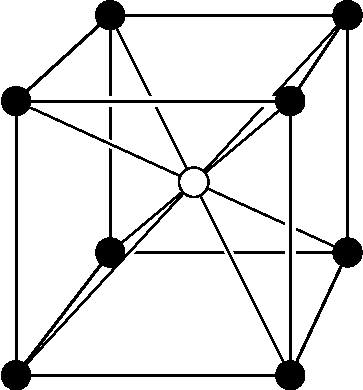
\includegraphics[width=0.4\linewidth]{fyz_fig738a.pdf}}               &
        \subfloat[ ]{\label{fyz_fig738b}
          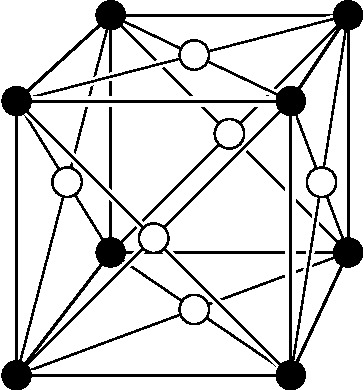
\includegraphics[width=0.4\linewidth]{fyz_fig738b.pdf}} 
      \end{tabular}
      \label{fyz_fig738}
      \caption{Elementární buňka krychlového krystalu a) prostorově centrovaná, b) plošně centrovaná
               (\cite[s.~547]{Feynman02})}
    \end{figure}
    
    Jak takové druhy krystalů vznikají? Představme si, že máme za úkol uspořádat sférické atomy 
    navzájem tak těsně, jak je to je m možné. Jeden způsob by byl udělat první vrstvu 
    šestiúhelníkového uspořádání, jak je znázorněno na obr. \ref{fyz_fig739a}. Pak můžeme vybudovat 
    druhou vrstvu podobně jako první, ale horizontálně posunutou (obr.\ref{fyz_fig739b}). Dále 
    můžete uložit třetí vrstvu. Ale pozor! Existují dva různé způsoby, jak umístit třetí vrstvu. 
    Začneme-li vytvářet třetí vrstvu tak, že umístíme atom do polohy \(A\) (obr. 
    \ref{fyz_fig739b}), bude každý atom v třetí vrstvě přímo nad atomem nejspodnější vrstvy. Když 
    však začneme třetí vrstvu vytvářet tak, že uložíme atom do polohy \(B\), budou atomy ve třetí 
    vrstvě mít svůj střed přesně nad bodem, který je středem trojúhelníka vytvořeného třemi atomy 
    spodní vrstvy. Každé jiné počáteční umístění je ekvivalentní buď s \(A\), nebo s \(B\), takže 
    jsou jen dva způsoby umístění třetí vrstvy.
    
    \begin{figure}[ht!]    %\ref{fyz_fig739}
      \centering
      \begin{tabular}{cc}
        \subfloat[ ]{\label{fyz_fig739a}
          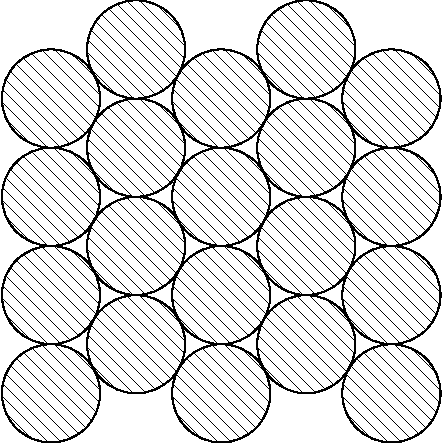
\includegraphics[width=0.4\linewidth]{fyz_fig739a.pdf}}               &
        \subfloat[ ]{\label{fyz_fig739b}
          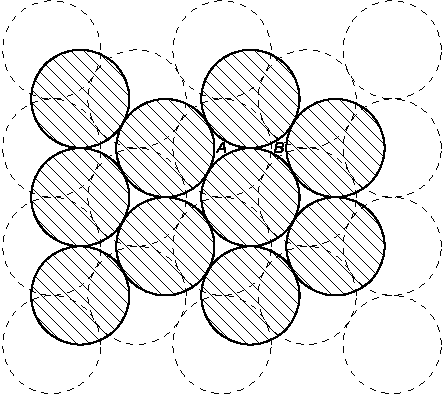
\includegraphics[width=0.4\linewidth]{fyz_fig739b.pdf}} 
      \end{tabular}
      \label{fyz_fig739}
      \caption{Budování těsně uspořádané šestiúhleníkové mřížky
               (\cite[s.~548]{Feynman02})}
    \end{figure}

    Má-li třetí vrstva atom v bodě \(B\), je to plošně centrovaná krychlová mřížka – ale viděná pod 
    určitým úhlem. Vypadá to divně, že jsme začali šestiúhelníky a skončili jsme krychlemi. 
    Všimněme si však, že díváme-li se na krychli z jednoho vrcholu, vidíme šestiúhelníkové obrysy. 
    Například obr. \ref{fyz_fig740} by mohl představovat rovinný šestiúhelník nebo krychli viděnou 
    z perspektivy.
    
    \begin{figure}[ht!] %\ref{fyz_fig740}
      \centering
      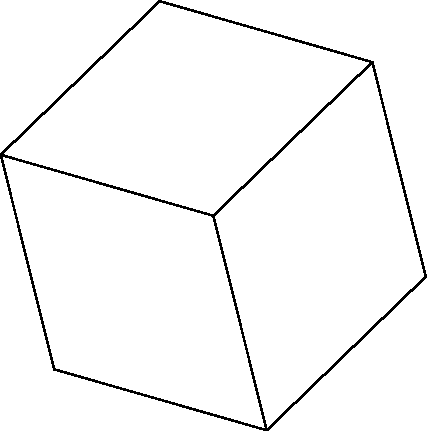
\includegraphics[width=0.4\linewidth]{fyz_fig740.pdf}
      \caption{Je toto šestiúhelník nebo krychle při pohledu z jejího vrcholu?
               (\cite[s.~548]{Feynman02})}
      \label{fyz_fig740}
    \end{figure}
    
    Doplníme-li třetí vrstvu na obr. \ref{fyz_fig739b} tak, že začneme s atomem v \(A\), 
    nedostaneme krychlovou strukturu, ale místo toho má mřížka jen šesterečnou symetrii. Je zřejmé, 
    že obě možnosti, které jsme popsali, představují stejně těsné uspořádání.
    
    Některé kovy, například měď nebo stříbro, si vybírají první alternativu-plošně centrovanou 
    krychli. Jiné, například berylium a hořčík, volí jiné alternativy - vytvářejí šesterečné 
    krystaly. Je zřejmé, že to, jaký krystal se vytvoří, nezávisí jen na uspořádání malých kuliček, 
    ale musí to být částečně určeno i jinými faktory. Konkrétně je to malá úhlová závislost 
    meziatomových sil (nebo v případě kovů závislost na energii elektronové „nádrže“). Tohle 
    všechno se dozvíme na přednáškách z chemie.
    
  \section{Symetrie ve dvou rozměrech}\label{fyz:IIchapXXXsecV}
    Nyní bychom chtěli pohovořit o některých vlastnostech krystalů z hlediska jejich vnitřních 
    symetrií. Hlavním rysem krystalů je ta vlastnost, že když se přemístíme o jednu mřížkovou 
    jednotku od jednoho atomu k příslušnému dalšímu, budeme opět v témže prostředí. To je základní 
    předpoklad. Ale kdybychom byli atomem, byl by tu ještě jiný druh změny, která by nás dostala 
    opět do téhož prostředí, tj. jiná možná symetrie. Na obr. \ref{fyz_fig741a} je znázorněn další 
    možný „tapetový“ vzor. Předpokládejme, že porovnáme okolí bodů \(A\) a \(B\). Na první pohled 
    se nám může zdát, že jsou stejná - ale ne docela. Body \(C\) a \(D\) jsou ekvivalentní s bodem 
    \(A\), ale okolí bodu \(B\) je jako okolí bodu \(A\) jen tehdy, převrátíme-li jej, tj. v 
    zrcadlovém obrazu.

    \begin{figure}[ht!]    %\ref{fyz_fig741}
      \centering
      \begin{tabular}{c}
        \subfloat[ ]{\label{fyz_fig741a}
          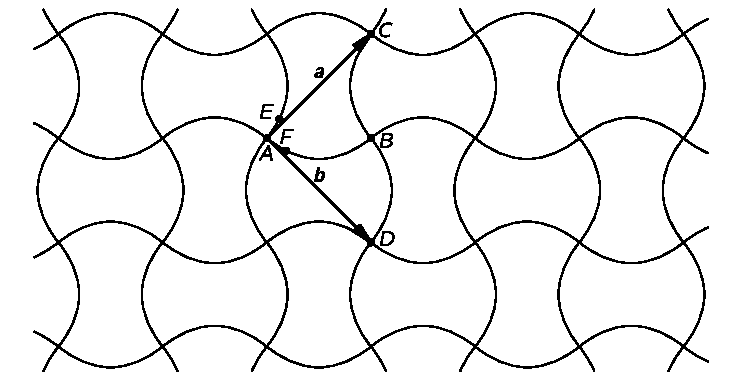
\includegraphics[width=0.9\linewidth]{fyz_fig741a.pdf}}               \\
        \subfloat[ ]{\label{fyz_fig741b}
          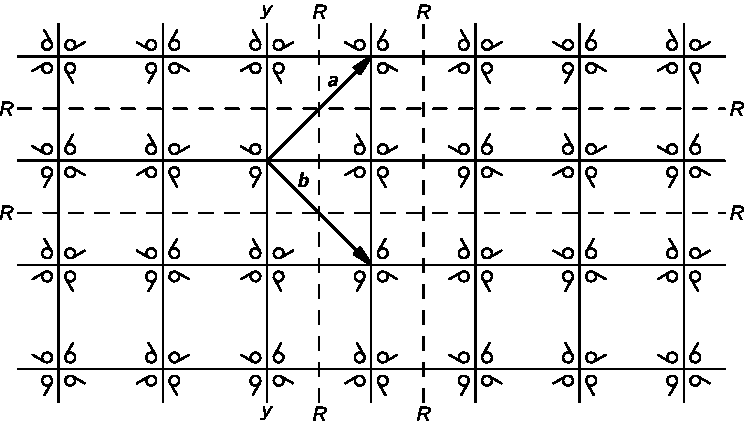
\includegraphics[width=0.9\linewidth]{fyz_fig741b.pdf}} 
      \end{tabular}
      \caption{Vzory s vyšší symetrií
               (\cite[s.~549]{Feynman02})}
      \label{fyz_fig741}
    \end{figure}

    V tomto vzoru jsou další druhy ekvivalentních bodů. Například body \(E\) a \(F\) mají stejné 
    okolí až na to, že jsou vzájemně otočeny o \SI{90}{\degree}. Rotace o úhel \SI{90}{\degree} 
    (nebo jeho libovolný násobek) kolem vrcholů, jako je \(A\), vede všude opět k témuž vzoru. 
    Krystal s takovouto strukturou je navenek pravoúhlý, ale uvnitř je komplikovanější než 
    jednoduchá krychle. Nyní, když jsme popsali některé speciální případy, pokusíme se přijít na 
    všechny možné symetrie, které může krystal mít. Nejdříve uvažujme, co se stane v rovině. 
    Rovinná mřížka může být definována dvěma \emph{základními} vektory, které mají počátek v jednom 
    bodě mřížky a koncové body ve dvou \emph{nejbližších} ekvivalentních bodech. Dva vektory 
    \(\bm{1}\) a \(\bm{2}\) jsou základními vektory mřížky na obr. \ref{fyz_fig733}. Dva vektory 
    \(\bm{a}\) a \(\bm{b}\) na obr. \ref{fyz_fig741a} jsou základními vektory znázorněného vzoru. 
    Mohli bychom, samozřejmě, vybrat \(\bm{-a}\) místo \(\bm{b}\) nebo \(\bm{-b}\) místo 
    \(\bm{a}\). Jelikož \(\bm{a}\) a \(\bm{b}\) mají stejnou velikost a jsou na sebe kolmé, přejde 
    při rotaci o \SI{90}{\degree} \(\bm{a}\) do \(\bm{b}\) a \(\bm{b}\) do \(\bm{-a}\), což nám 
    dává opět tutéž mřížku. Vidíme, že existují mřížky, které mají „čtyřstrannou“ symetrii. A před 
    tím jsme popsali těsné uspořádání založené na šestiúhelnících, které by mohlo mít 
    „šestistrannou“ symetrii. Seskupení kružnic na obr. \ref{fyz_fig739a} se při rotaci o 
    \SI{60}{\degree} kolem středu libovolné kružnice zobrazuje opět tentýž vzor. Jaké jiné druhy 
    rotační symetrie ještě existují? Můžeme mít například pětinásobné nebo osminásobné rotační 
    symetrie? Lze snadno vidět, že tyto jsou vyloučeny.\emph{ Jedinou symetrií, založenou na útvaru 
    s více než čtyřmi stranami, je šestistranná symetrie}. Nejdříve ukážeme, že symetrie s více než 
    šesti stranami je vyloučena. Zkusme si představit mřížku se dvěma stejně velkými základními 
    vektory, které svírají úhel menší než \SI{60}{\degree} (obr. \ref{fyz_fig742a}). Předpokládáme, 
    tedy, že body \(B\) a \(C\) jsou ekvivalentní s bodem \(A\) a že \(\bm{a}\) a \(\bm{b}\) jsou 
    dva nejkratší vektory od \(A\) k jeho ekvivalentním sousedům. To je však zřejmě nesprávné, 
    neboť vzdálenost mezi body \(B\) a \(C\) je menší než vzdálenost libovolného z nich od \(A\). 
    Musí tu být nějaký soused \(D\), který je ekvivalentní s \(A\) a je k němu blíže než \(B\) nebo 
    \(C\). Měli bychom zvolit \(\bm{b'}\) za jeden z našich základních vektorů. Proto úhel mezi 
    dvěma základními vektory musí být \SI{60}{\degree} nebo více. Osmiúhelníková symetrie není 
    možná.

    A co takhle pětinásobná symetrie? Předpokládáme-li, že základní vektory \(\bm{a}\) a \(\bm{b}\) 
    mají stejné délky a svírají úhel \(2\pi /5 = \SI{72}{\degree}\) (obr. \ref{fyz_fig742b}), měl 
    by existovat ekvivalentní mřížkový bod \(D\) odkloněný o \SI{72}{\degree} od \(C\). Ale vektor 
    \(\bm{b'}\) směřující od \(E\) do \(D\) je menší než \(\bm{b}\), proto \(\bm{b}\) není 
    základním vektorem. Pětinásobná symetrie nemůže existovat. Jediné možnosti, které nás 
    nepřivedou do těchto obtíží jsou \(\vartheta = \SI{60}{\degree}; \SI{90}{\degree}\) nebo 
    \SI{120}{\degree}. Nula nebo \SI{180}{\degree} jsou také zřejmě možné. Náš výsledek lze 
    zformulovat i tak, že vzor může zůstávat nezměněn při rotaci o celých \SI{360}{\degree} (vůbec 
    žádná změna), o jednu polovinu, jednu třetinu, jednu čtvrtinu nebo jednu šestinu celé otáčky. A 
    to jsou všechny možné rotační symetrie v rovině - celkem pět. Je-li \(\vartheta = 2\pi/n\), 
    mluvíme o \(n\)-násobné symetrii. Říkáme, že vzor s \(n\) rovným \(4\) nebo \(6\) má vyšší 
    symetrii než vzor s \(n\) rovným \(1\) nebo \(2\). 

    \begin{figure}[ht!]    %\ref{fyz_fig742}
      \centering
      \begin{tabular}{c}
        \subfloat[ ]{\label{fyz_fig742a}
          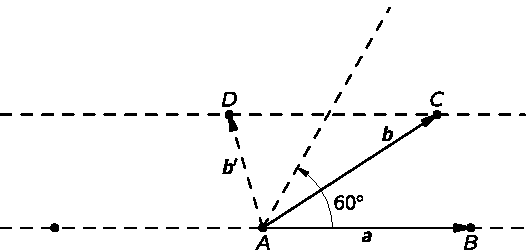
\includegraphics[width=0.9\linewidth]{fyz_fig742a.pdf}}               \\
        \subfloat[ ]{\label{fyz_fig742b}
          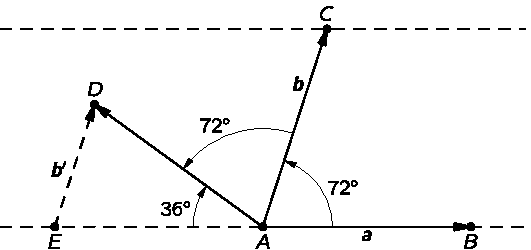
\includegraphics[width=0.9\linewidth]{fyz_fig742b.pdf}} 
      \end{tabular}
      \caption{a) Rotační symetrie vyšší než šestinásobné nejsou možné. b) Pětinásobná symetrie 
               není možná.
               (\cite[s.~550]{Feynman02})}
      \label{fyz_fig742}
    \end{figure}

    Vraťme se k obr. \ref{fyz_fig741a}. Vidíme, že vzor má čtyřnásobnou rotační symetrii. Na obr. 
    \ref{fyz_fig741b} jsme nakreslili jiný vzor, který má tytéž vlastnosti symetrie jako obr. 
    \ref{fyz_fig741a}. Malé značky podobné čárkám jsou asymetrické objekty, které nám slouží k 
    určení symetrie vzoru uvnitř každého čtverečku. Všimněme si, že čárky v sousedních čtvercích 
    jsou převrácené, takže základní buňka je větší než jeden čtvereček. Kdyby nebyly čárky, měl by 
    vzor také čtyřnásobnou symetrii, ale základní buňka by byla menší. Vzor na obr. 
    \ref{fyz_fig741} má ještě další druhy symetrie. Například při zrcadlovém zobrazení vzhledem k 
    přerušovaným osám \(\bm{R} \rightarrow \bm{-R}\) dostaneme tentýž vzor. 

    A ještě je tu jeden druh symetrie pro vzor na obr. \ref{fyz_fig741}. Provedeme-li zrcadlový 
    obraz vzhledem k ose \(Y-Y\) \emph{plus} posun o jeden čtvereček doprava (nebo doleva), 
    dostaneme opět původní vzor. Čára \(Y-Y\) se nazývá \textbf{skluzná čára}.

    To jsou všechny možné symetrie pro dva rozměry. V prostoru existuje ještě jedna operace 
    symetrie, jíž v \emph{dvojrozměrném} případě odpovídá rotace o \SI{180}{\degree}, ale ve třech 
    rozměrech je to zcela odlišná operace. Je to \emph{inverze}. Inverzí rozumíme přemístění bodu, 
    jehož polohový vektor je \(\bm{R}\), do bodu \(\bm{-R}\) (obr. \ref{fyz_fig743b}). 

    \begin{figure}[ht!]   %\ref{fyz_fig743}
      \centering
      \begin{tabular}{cc}
        \subfloat[ ]{\label{fyz_fig743a}
          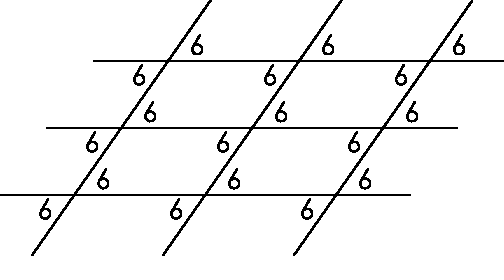
\includegraphics[width=0.45\linewidth]{fyz_fig743a.pdf}}               &
        \subfloat[ ]{\label{fyz_fig743b}
          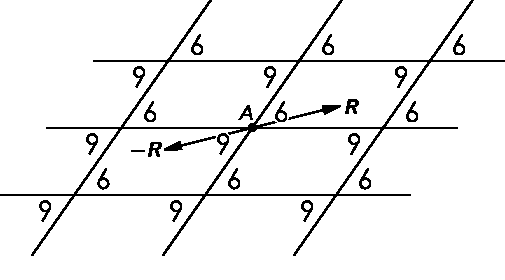
\includegraphics[width=0.45\linewidth]{fyz_fig743b.pdf}}              \\
        \subfloat[ ]{\label{fyz_fig743c}
          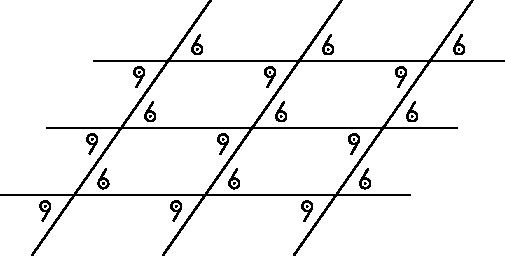
\includegraphics[width=0.45\linewidth]{fyz_fig743c.pdf}}               &
        \subfloat[ ]{\label{fyz_fig743d}
          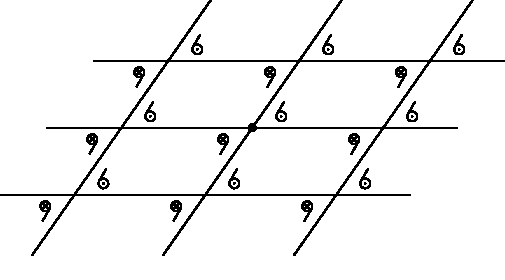
\includegraphics[width=0.45\linewidth]{fyz_fig743d.pdf}} 
      \end{tabular}
      \caption{Symetrie vzhledem k inverzi. Vzor b) zůstává nezměněn při \(\bm{R} \rightarrow 
               \bm{-R}\), ale vzor a) se mění. Trojrozměrný vzor d) je při inverzi symetrický, ale 
               c) není
               (\cite[s.~551]{Feynman02})}
      \label{fyz_fig743}
    \end{figure}

    Při inverzi vzoru na obr. \ref{fyz_fig743a} dostáváme nový vzor, ale při inverzi vzoru (obr. 
    \ref{fyz_fig743b}) se reprodukuje tentýž vzor. Pro dvojrozměrné vzory (jak vidíme na obrázku 
    \ref{fyz_fig743b}) je inverze vzoru vzhledem k bodu \(A\) ekvivalentní s rotací o 
    \SI{180}{\degree} kolem téhož bodu. Předpokládejme, že bychom vzor na obr. \ref{fyz_fig743b} 
    předělali na trojrozměrný tak, že bychom všechny malé znaky \num{6} a \num{9} doplnili šipkou 
    směřující ven z obrázku. Po inverzi v třech rozměrech by všechny šipky přešly na opačné, takže 
    by se vzor nereprodukoval. Označíme-li počátky šipek tečkami a konce křížky, můžeme sestavit 
    trojrozměrný vzor, jako je na obr. \ref{fyz_fig743c}, který není symetrický vzhledem k inverzi. 
    Můžeme také vytvořit vzor znázorněný na obr. \ref{fyz_fig743d}, který má takovou symetrii. 
    Všimněme si, že trojrozměrnou inverzi nelze nahradit nějakou kombinací rotací.

    Charakterizujeme-li symetrii vzoru - nebo mřížky - týmiž druhy operací symetrie, které jsme 
    popsali, lze ukázat, že ve dvojrozměrném případě může existovat \num{17} různých vzorů. Na obr. 
    \ref{fyz_fig733} jsme nakreslili vzor, který patří k vzorům s nejnižší symetrií, a na obr. 
    \ref{fyz_fig741} je ukázka vzoru s vyšší symetrií. S vymýšlením všech sedmnácti možných vzorů 
    si můžeme pohrát sami.
    
    Je zajímavé, jak málo vzorů ze všech \num{17} možných se používá při navrhování tapet a 
    textilních vzorů. Všude se setkáváme jen s týmiž třemi nebo čtyřmi základními vzory. Je to 
    nedostatek fantazie návrhářů, nebo je to proto, že ostatní vzory nelahodí oku?
    
  \section{Symetrie ve třech rozměrech}\label{fyz:IIchapXXXsecVI}
    Dosud jsme hovořili jen o dvojrozměrných vzorech. To, co nás však ve skutečnosti zajímá, je 
    uspořádání atomů ve třech rozměrech. Z prvé je zřejmé, že trojrozměrný krystal bude mít tři 
    základní vektory. Kdybychom se zeptali na možné operace symetrie ve třech rozměrech, zjistili 
    bychom, že existuje \num{230} různých možných symetrií. Z jistých důvodů rozdělujeme těchto 
    \num{230} typů na sedm tříd, které jsou znázorněny na obr. \ref{fyz_fig744}. Mřížka s nejnižší 
    symetrií se nazývá \textbf{trojklonná} Základní buňkou je \emph{rovnoběžnostěn}. Základní 
    vektory mají nestejné délky a žádné dva z úhlů, které navzájem svírají, nejsou stejné. Tato 
    mřížka nemá rotační symetrii ani symetrii odrazu. Dvě možné symetrie tu však přece jen jsou - 
    základní buňka je, nebo není změněna při inverzi vzhledem k jednomu vrcholu. (Inverzí v 
    trojrozměrném případě rozumíme záměnu vektoru posunutí \(\bm{R}\) na \(\bm{-R}\), jinými slovy 
    záměnu \((x, y, z)\) za \((-x, -y, -z)\).) Trojklonná mřížka má tedy jen dvě možné symetrie s 
    výjimkou případů, kdy základní vektory splňují určité speciální vztahy. Například jsou-li 
    všechny vektory stejné a svírají stejné úhly, dostáváme \textbf{klencovou} mřížku znázorněnou 
    na obrázku. Znázorněná buňka může mít ještě dodatečnou symetrii - může zůstat nezměněna při 
    rotaci kolem nejdelší, tělesové úhlopříčky.
    

    \begin{figure}[ht!]   %\ref{fyz_fig744}
      \centering
      \begin{tabular}{cc}
        \subfloat[ ]{\label{fyz_fig744a}
          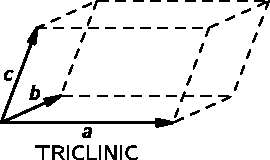
\includegraphics[width=0.4\linewidth]{fyz_fig744a.pdf}}               &
        \subfloat[ ]{\label{fyz_fig744b}
          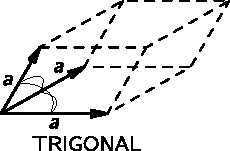
\includegraphics[width=0.4\linewidth]{fyz_fig744b.pdf}}              \\
        \subfloat[ ]{\label{fyz_fig744c}
          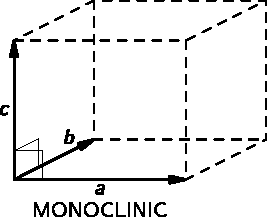
\includegraphics[width=0.4\linewidth]{fyz_fig744c.pdf}}               &
        \subfloat[ ]{\label{fyz_fig744d}
          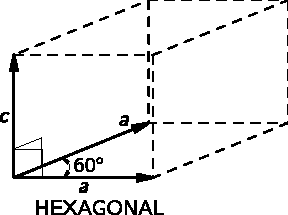
\includegraphics[width=0.4\linewidth]{fyz_fig744d.pdf}}               \\
        \subfloat[ ]{\label{fyz_fig744e}
          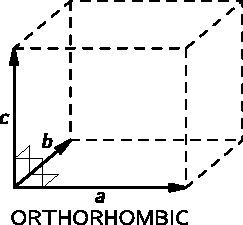
\includegraphics[width=0.4\linewidth]{fyz_fig744e.pdf}}               &
        \subfloat[ ]{\label{fyz_fig744f}
          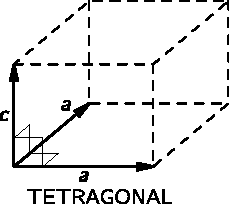
\includegraphics[width=0.4\linewidth]{fyz_fig744f.pdf}}               \\
        \subfloat[ ]{\label{fyz_fig744g}
          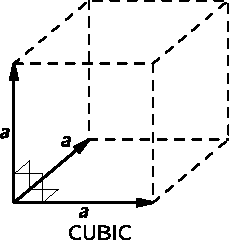
\includegraphics[width=0.4\linewidth]{fyz_fig744g.pdf}}
      \end{tabular}
      \caption{Sedm tříd krystalických mřížek
               (\cite[s.~552]{Feynman02})}
      \label{fyz_fig744}
    \end{figure}
    
    Je-li jeden ze základních vektorů, například \(\bm{c}\), kolmý na ostatní dva vektory, 
    dostáváme základní \textbf{jednoklonnou} buňku. Novou možnou symetrií je rotace o 
    \SI{180}{\degree} kolem \(\bm{c}\). Speciálním případem je \textbf{šesterečná} buňka, v níž 
    jsou vektory \(\bm{a}\) a \(\bm{b}\) stejné a svírají úhel \SI{60}{\degree}, takže při rotaci o 
    \SI{60}{\degree}, \SI{120}{\degree} nebo \SI{180}{\degree} kolem vektoru \(\bm{c}\) dostáváme 
    tutéž mřížku (pro určité vnitřní symetrie).
    
    Jsou-li všechny tři základní vektory navzájem kolmé, ale mají různou délku, dostáváme 
    \textbf{kosočtverečnou} buňku. Buňka je symetrická při rotacích o \SI{180}{\degree} kolem tří 
    os. Symetrie vyššího řádu má \textbf{čtverečná} buňka, která má všechny úhly pravé a dva její 
    základní vektory mají stejnou délku. Nakonec je tu \textbf{krychlová} mřížka, která je nejvíce 
    symetrická ze všech.
    
    Smyslem všech těchto úvah o symetriích je to, že vnitřní symetrie krystalů se projevují, někdy 
    jen nenápadným způsobem, v makroskopických fyzikálních vlastnostech krystalu. Obecně je 
    například elektrická polarizovatelnost krystalu charakterizována tenzorem. Vyjádříme-li tento 
    tenzor pomocí elipsoidu polarizace, lze předpokládat, že tento elipsoid bude odrážet některé 
    vlastnosti symetrie krystalu. Například krychlový krystal je symetrický vzhledem k rotacím o 
    \SI{90}{\degree} kolem libovolné ze tří kolmých os. Je zřejmé, že jediný elipsoid s touto 
    vlastností je \emph{koule}. \emph{Krychlový krystal musí být izotropním dielektrikem}.
    
    Na druhé straně čtverečný krystal má čtyřnásobnou rotační symetrii. Jeho elipsoid musí mít dvě 
    z hlavních os stejné a třetí musí být rovnoběžná s osou krystalu. Podobně kosočtverečný 
    krystal, protože má dvojnásobnou rotační symetrii vzhledem ke třem navzájem kolmým osám, musí 
    mít osy totožné s osami elipsoidu polarizace. Podobně jedna z os jednoklonného krystalu musí 
    být rovnoběžná s jednou z hlavních os elipsoidu, ale o jeho dalších osách nemůžeme nic říci. 
    Protože trojklonný krystal nemá žádnou rotační symetrii, může být jeho elipsoid orientován 
    libovolně.
    
    Jak vidíme, mohli bychom si do nekonečna hrát s výčtem různých symetrií a určováním jejich 
    vztahu k různým fyzikálním tenzorům. Uvažovali jsme jen tenzor polarizovatelnosti, ale i s 
    jinými tenzory (například tenzorem pružnosti) je to komplikovanější. Existuje matematický obor 
    nazývaný teorie grup, který se těmito otázkami zabývá, ale obvykle se lze dopracovat k výsledku 
    jen na základě zdravého rozumu.
    
  \section{Pevnost kovů}\label{fyz:IIchapXXXsecVII}
    Řekli jsme si, že kovy mají obvykle krychlovou krystalickou strukturu. Nyní budeme hovořit o 
    jejich mechanických vlastnostech, které závisejí na této struktuře, Kovy jsou obecně velmi 
    „měkké“, neboť lze snadno posouvat jednu vrstvu krystalu vzhledem k druhé. Možná si řeknete: 
    „Vždyť je to nesmysl, kovy jsou přece pevné!“ Není to tak. \emph{Jednotlivé krystaly} kovu 
    můžeme snadno deformovat.
    
    \begin{figure}[ht!]    %\ref{fyz_fig745}
      \centering
      \begin{tabular}{c}
        \subfloat[ ]{\label{fyz_fig745a}
          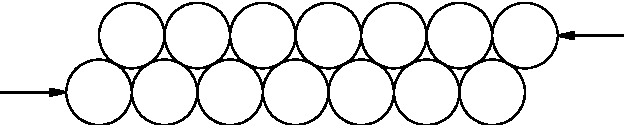
\includegraphics[width=0.7\linewidth]{fyz_fig745a.pdf}}               \\
        \subfloat[ ]{\label{fyz_fig745b}
          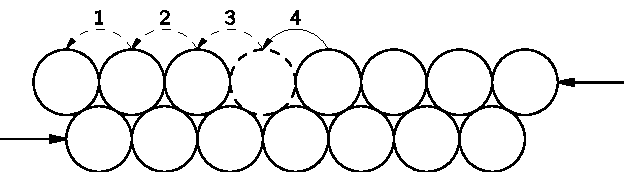
\includegraphics[width=0.7\linewidth]{fyz_fig745b.pdf}} 
      \end{tabular}
      \caption{Skluz krystalových rovin
               (\cite[s.~552]{Feynman02})}
      \label{fyz_fig745}
    \end{figure}
    
    Podívejme se na dvě vrstvy krystalu, na které působí smyková síly (obr. \ref{fyz_fig745a}). Na 
    první pohled se může zdát, že celá vrstva bude odolávat působení, dokud nebude síla dostatečně 
    velká na to, aby pohnula celou vrstvou „přes hrboly“, takže ta se posune o jedno místo doleva. 
    Ačkoli posun se vztahuje na celou rovinu, neprobíhá to tímto způsobem. (Kdyby to tak bylo, 
    vyšlo by vám, že kov má být mnohem pevnější, než ve skutečnosti je..) Spíše je to tak, jakoby 
    se atomy přemisťovaly jeden po druhém. Nejdříve poskočí atom, který je úplně nalevo, potom 
    další atd., jak je znázorněno na obr. \ref{fyz_fig745b}. Celkový efekt je takový, že prázdné 
    místo mezi dvěma atomy putuje rychle směrem doprava, až se nakonec celá vrstva přemístí o jednu 
    meziatomovou vzdálenost. Posun probíhá tímto způsobem proto, že se spotřebuje méně energie při 
    přesunutí jednoho atomu přes hrbol než při přesunu celé řady. Jakmile je síla dostatečně velká, 
    může proces začít a zbytek už postupuje velmi rychle.
    
    
    \begin{figure}[ht!] %\ref{fyz_fig746}
      \centering
      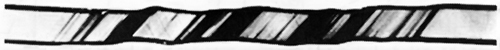
\includegraphics[width=0.7\linewidth]{fyz_fig746.jpg}
      \caption{Fotografie malého krystalu mědi po natažení (S dovolením S. S. Brennera, vědeckého 
               pracovníka Ocelářského výzkumného centra, Monroeville, Pensylvánie, USA.)
               (\cite[s.~552]{Feynman02})}
      \label{fyz_fig746}
    \end{figure}
    
    Ukazuje se, že ve skutečném krystalu probíhá posouvání opakovaně v jedné rovině, pak se zastaví 
    a začne v nějaké jiné rovině. Detailní zdůvodnění, proč proces začne a proč končí, zůstává 
    záhadou. Je vlastně velmi divné, že oblasti, v nichž posun postupně probíhá, bývají od sebe 
    přibližně stejně vzdáleny. Na obr. \ref{fyz_fig746} je fotografie malého tenkého krystalu mědi, 
    který byl „natahován“. Můžeme rozeznat různé roviny, v nichž nastalo posunutí.
    
    O náhlém posunu jednotlivých rovin krystalu se můžeme přímo přesvědčit. Vezmeme-li si kousek 
    tenkého drátku, který obsahuje velké krystaly, a napneme jej v blízkosti ucha, můžeme slyšet 
    „tikot“ provázející postupné zapadání rovin do svých nových poloh. 
    
    Problém „chybějícího“ atomu v řadě je o něco složitější, než se zdá z obr. \ref{fyz_fig745}. 
    Máme-li víc vrstev, vznikne podobná situace jako na obr. \ref{fyz_fig747}. 
    
    \begin{figure}[ht!] %\ref{fyz_fig747}
      \centering
      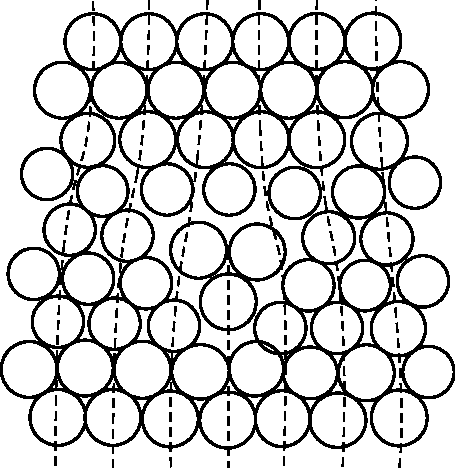
\includegraphics[width=0.7\linewidth]{fyz_fig747.pdf}
      \caption{Dislokace v krystalu
               (\cite[s.~554]{Feynman02})}
      \label{fyz_fig747}
    \end{figure}

    Taková nedokonalost v krystalu se nazývá \textbf{dislokace}. Předpokládá se, že dislokace jsou 
    buď přítomny v krystalu už při jeho formování, nebo se vytvoří u nějaké trhliny nebo zářezu na 
    povrchu. Když už jednou vzniknou, mohou se v krystalu poměrně volně pohybovat. Při pohybu 
    takovýchto dislokací vznikají větší deformace.
    
    Dislokace se mohou volně pohybovat, to znamená, že k tomu stačí malá dodatečná energie za 
    předpokladu, že zbytek krystalu je dokonalou mřížkou. Ale mohou se „zaseknout“, když se setkají 
    s nějakým jiným druhem defektu v krystalu. Je-li třeba velké energie k tomu, aby se dislokace 
    přes defekt dostaly, zastaví se. To je právě mechanizmus, který je příčinou pevnosti 
    nedokonalých kovových krystalů. Čisté krystaly železa jsou docela měkké, ale malá koncentrace 
    atomů příměsi může vyvolat tolik poruch, že dislokace budou efektivně znehybněny. Jak víme, 
    ocel, která je převážně železem, je velmi tvrdá. Při výrobě oceli se malé množství uhlíku 
    rozpustí v roztaveném železe. Při rychlém ochlazení vytvářejí zrníčka uhlíku v mřížce množství 
    mikroskopických poruch. Dislokace se už nemohou volně pohybovat a kov se stane pevným.
    
    \begin{figure}[ht!] %\ref{fyz_fig748}
      \centering
      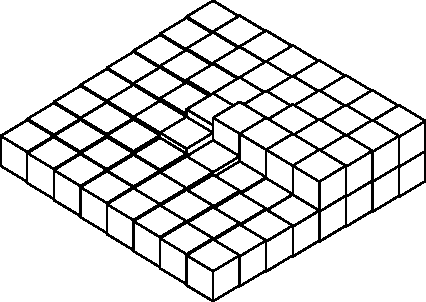
\includegraphics[width=0.7\linewidth]{fyz_fig748.pdf}
      \caption{Dislokace v torzi (Z knihy Ch. Kittel: Úvod do fyziky pevných látek, v českém 
               překladu vyšlo v nakladatelství Academia, Praha 1985.)
               (\cite[s.~554]{Feynman02})}
      \label{fyz_fig748}
    \end{figure}
    
    Čistá měď je velmi měkká, ale může ji udělat tvrdší tím, že ji ohýbáme, nebo vyklepeme 
    kladivem. V tomto případě se vytváří mnoho nových dislokací různých druhů, které navzájem 
    interferují, a tak omezují svou pohyblivost. Vezměme kousek měkké mědi a snadno jej obtočíme 
    někomu kolem zápěstí jako náramek. Přitom se měď zpevní a my ji nemůžeme ohnout nazpět! 
    Mechanicky zpevněné kovy typu mědi můžeme udělat opět měkkým žíháním při vysoké teplotě. 
    Tepelným pohybem atomů se \uv{vyžehlí} dislokace a vytvoří se opět jednotlivé velké krystaly. 
    Dosud jsme popisovali jen dislokace ve \emph{smyku}. Existuje ještě mnoho jiných druhů 
    dislokací, z nichž jedna, dislokace v\emph{torzi} je znázorněná na obr. \ref{fyz_fig748}. 
    Takové dislokace často hrají důležitou úlohu při růstu krystalů. 
    
  \section{Dislokace a růst krystalů}\label{fyz:IIchapXXXsecVIII}
    Proces růstu krystalů byl dlouhou dobu velkou záhadou. Už jsme hovořili o tom, jak každý atom 
    může opakovaným zkoušením určit, zda je lepší být v krystalu nebo mimo něj. Ale to znamená, že 
    každý atom musí najít místo s nejnižší energií. Avšak atom, který dopadne na nový povrch, je 
    zespoda vázán jen jednou - dvěma vazbami a nemá tutéž energii, kterou by měl, kdyby byl umístěn 
    někde v rohu, obklopen ze tří stran. Představme si rostoucí krystal jako blok sestavovaný z 
    kostek, jak vidíme na obr. \ref{fyz_fig749}. Pokusíme-li se přidat novou kostku, řekněme do 
    polohy \(A\), bude mít tato kostka jen jednoho ze šesti možných sousedů, kterými by se nakonec 
    obklopila. Při tolika chybějících vazbách nemůže být energie příliš nízká. Výhodnější by byla 
    poloha \(B\), kde je až polovina vazeb nasycena. A skutečně, krystaly rostou tak, že nové atomy 
    se připojují v místech, jako je \(B\).
    
    \begin{figure}[ht!] %\ref{fyz_fig749}
      \centering
      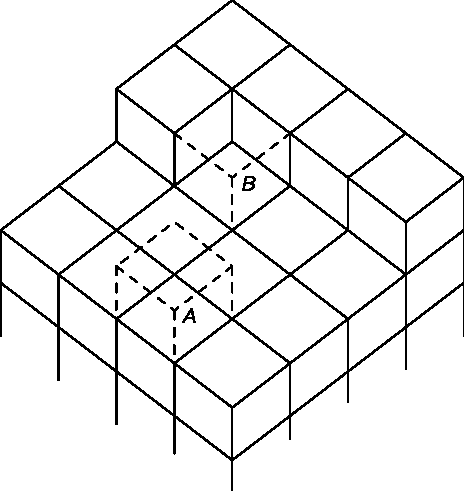
\includegraphics[width=0.6\linewidth]{fyz_fig749.pdf}
      \caption{Růst krystalu
               (\cite[s.~555]{Feynman02})}
      \label{fyz_fig749}
    \end{figure}

    Co se však stane, je-li jedna řada ukončena? K započetí nové řady se musí atom usadit v poloze, 
    v níž je připojen jen ze dvou stran, a to je dost nepravděpodobné. I kdyby se to stalo, co bude 
    pak, když se ukončí celá vrstva? Jak může začít nová vrstva? Jedna z možných odpovědí je, že 
    pro krystal je nejvýhodnější růst v místech dislokace, například v okolí dislokace v torzi 
    podobné té, která je na obr. \ref{fyz_fig748}. V takovém krystalu se při přidávání nové kostky 
    vždy najde místo se třemi dostupnými vazbami. V krystaluje tedy zvýhodněn růst se zabudovanou 
    dislokací. Příklad takovéhoto spirálového růstu je na obr. \ref{fyz_fig750}, který je 
    fotografií monokrystalu parafínu.
    
    \begin{figure}[ht!] %\ref{fyz_fig750}
      \centering
      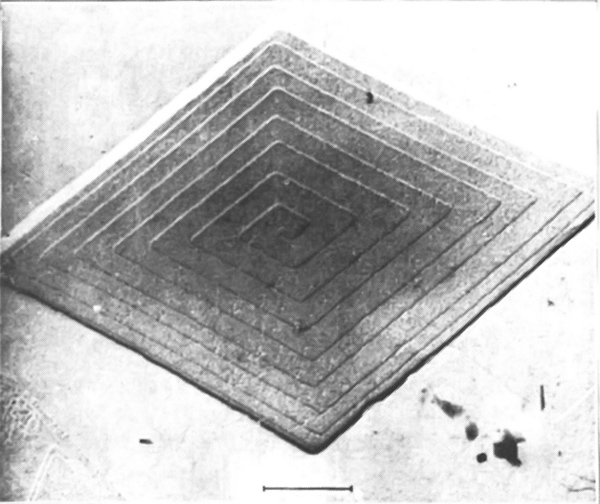
\includegraphics[width=0.7\linewidth]{fyz_fig750.jpg}
      \caption{Krystal parafínu, který vyrostl v okolí dislokace v torzi
               (\cite[s.~555]{Feynman02})}
      \label{fyz_fig750}
    \end{figure}

  \section{Braggův-Nyeův model krystalu}\label{fyz:IIchapXXXsecIX}
    Samozřejmě nemůžeme vidět, co se děje sjednotlivými atomy v krystalu. Jak už nyní sami vidíte, 
    v krystalu existuje mnoho komplikovaných jevů, které nelze jednoduše kvantitativně popsat. Sir 
    Lawrence Bragg a J. F. Nye navrhli schéma sestrojení modelu kovového krystalu. Je překvapující, 
    že v rámci tohoto modelu lze odvodit jevy, které, zdá se, vznikají ve skutečných krystalech. Na 
    následujících stránkách reprodukujeme jejich původní článek, v němž je popsána jejich metoda a 
    jsou uvedeny některé výsledky, které její pomocí získali. (Článek je převzat z Proceeding of 
    the Royal Society od London, Vol 190, září 1947, s. 474 až 481 - s povolením autorů a Královské 
    společnosti.)

    \begin{figure}[ht!] %\ref{fyz_fig751}
      \centering
      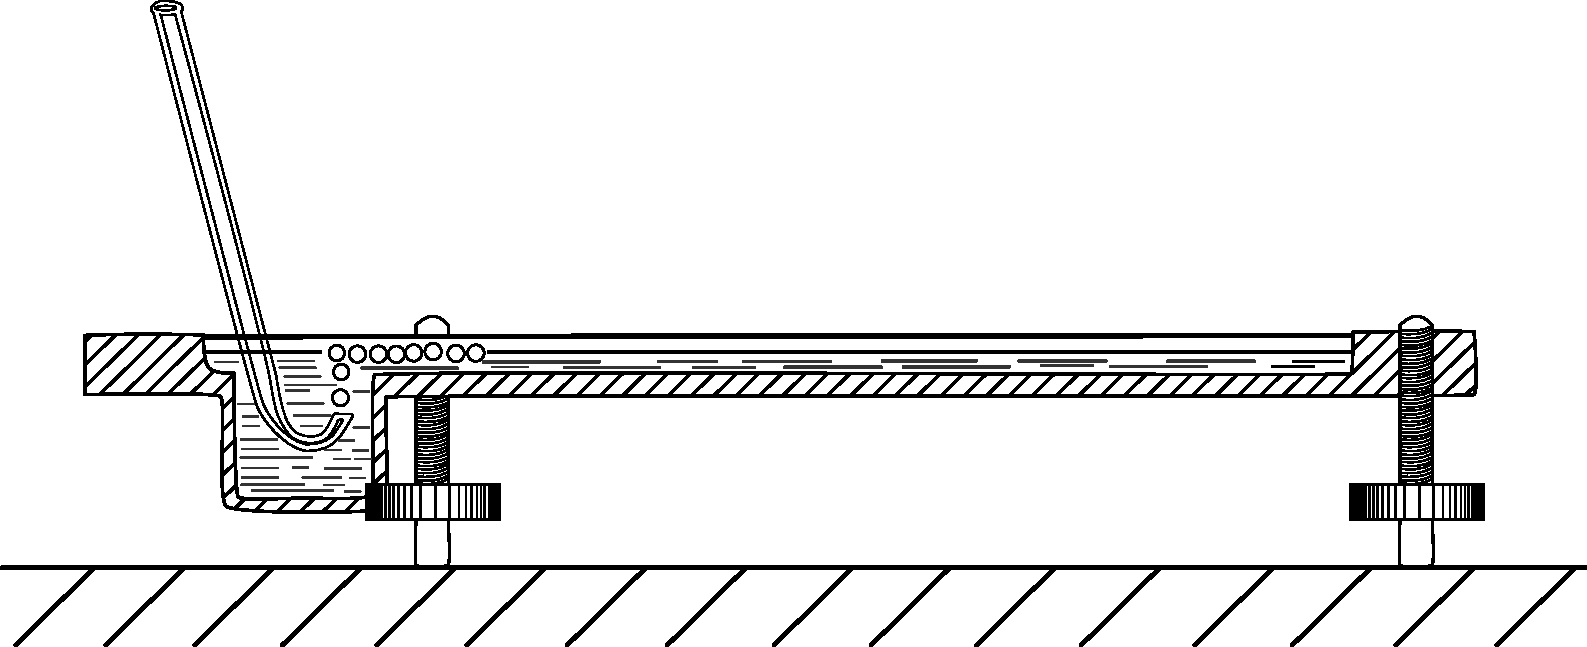
\includegraphics[width=0.7\linewidth]{fyz_fig751.pdf}
      \caption{Přístroj na výrobu bublinových vrstev
               (\cite[s.~557]{Feynman02})}
      \label{fyz_fig751}
    \end{figure}

    \begin{figure}[ht!] %\ref{fyz_fig752}
      \centering
      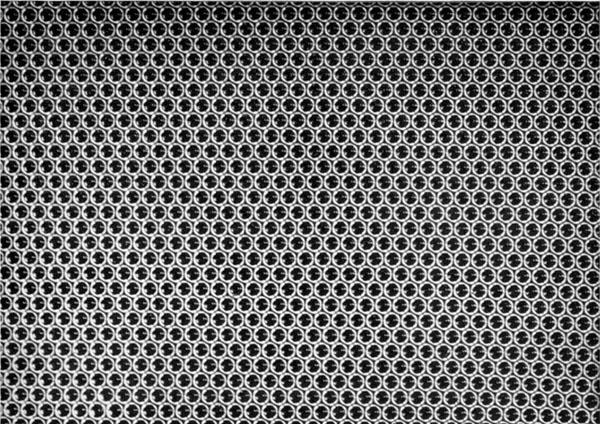
\includegraphics[width=0.7\linewidth]{fyz_fig752.jpg}
      \caption{
               (\cite[s.~707]{Feynman02})}
      \label{fyz_fig752}
    \end{figure}

    \begin{figure}[ht!] %\ref{fyz_fig753}
      \centering
      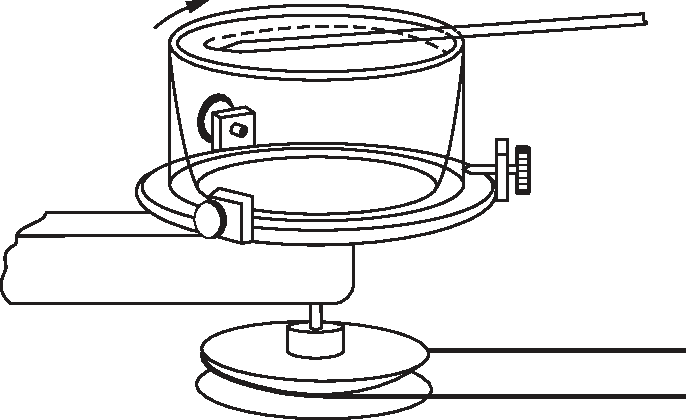
\includegraphics[width=0.7\linewidth]{fyz_fig753.pdf}
      \caption{
               (\cite[s.~707]{Feynman02})}
      \label{fyz_fig753}
    \end{figure}



    \begin{figure}[ht!] %\ref{fyz_fig754}
      \centering
      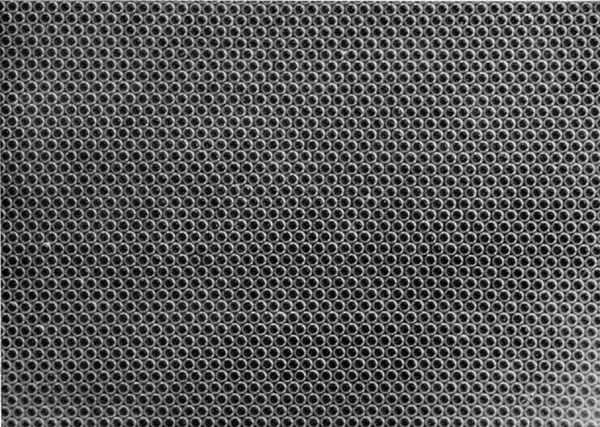
\includegraphics[width=0.7\linewidth]{fyz_fig754.jpg}
      \caption{
               (\cite[s.~707]{Feynman02})}
      \label{fyz_fig754}
    \end{figure}

    \begin{figure}[ht!] %\ref{fyz_fig755}
      \centering
      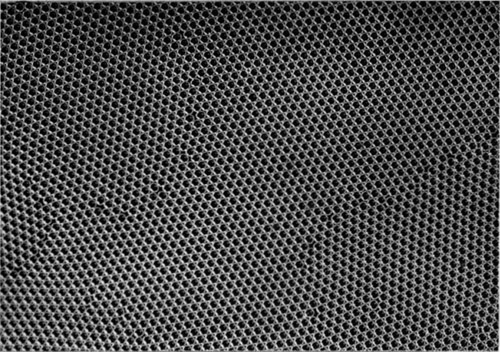
\includegraphics[width=0.7\linewidth]{fyz_fig755.jpg}
      \caption{
               (\cite[s.~707]{Feynman02})}
      \label{fyz_fig755}
    \end{figure}

    \begin{figure}[ht!] %\ref{fyz_fig756}
      \centering
      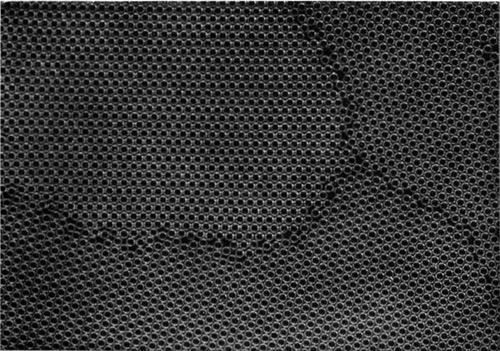
\includegraphics[width=0.7\linewidth]{fyz_fig756.jpg}
      \caption{
               (\cite[s.~707]{Feynman02})}
      \label{fyz_fig756}
    \end{figure}

    \begin{figure}[ht!] %\ref{fyz_fig757}
      \centering
      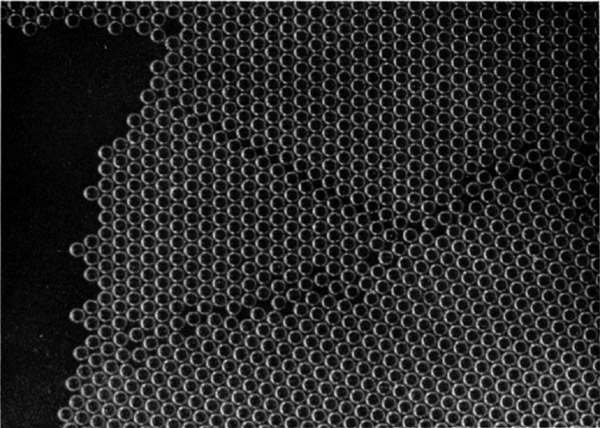
\includegraphics[width=0.7\linewidth]{fyz_fig757.jpg}
      \caption{
               (\cite[s.~707]{Feynman02})}
      \label{fyz_fig757}
    \end{figure}

    \begin{figure}[ht!] %\ref{fyz_fig758}
      \centering
      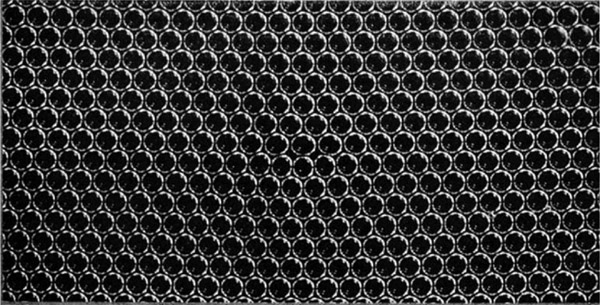
\includegraphics[width=0.7\linewidth]{fyz_fig758.jpg}
      \caption{
               (\cite[s.~707]{Feynman02})}
      \label{fyz_fig758}
    \end{figure}

    \begin{figure}[ht!] %\ref{fyz_fig759}
      \centering
      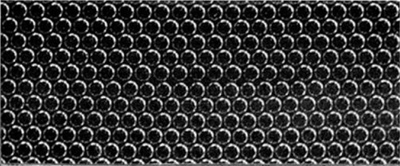
\includegraphics[width=0.7\linewidth]{fyz_fig759.jpg}
      \caption{
               (\cite[s.~707]{Feynman02})}
      \label{fyz_fig759}
    \end{figure}
    
    \begin{figure}[ht!] %\ref{fyz_fig760}
      \centering
      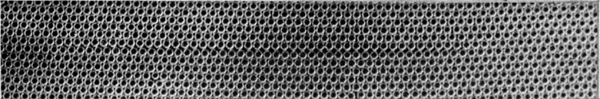
\includegraphics[width=0.7\linewidth]{fyz_fig760.jpg}
      \caption{
               (\cite[s.~707]{Feynman02})}
      \label{fyz_fig760}
    \end{figure}

    \begin{figure}[ht!] %\ref{fyz_fig761}
      \centering
      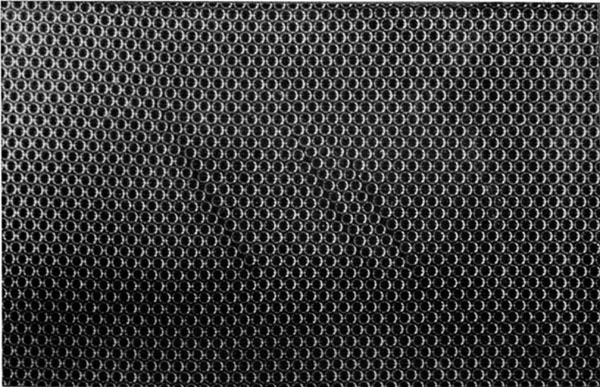
\includegraphics[width=0.7\linewidth]{fyz_fig761.jpg}
      \caption{
               (\cite[s.~707]{Feynman02})}
      \label{fyz_fig761}
    \end{figure}

    \begin{figure}[ht!] %\ref{fyz_fig762}
      \centering
      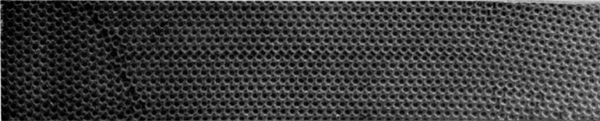
\includegraphics[width=0.7\linewidth]{fyz_fig762.jpg}
      \caption{
               (\cite[s.~707]{Feynman02})}
      \label{fyz_fig762}
    \end{figure}

    \begin{figure}[ht!] %\ref{fyz_fig763}
      \centering
      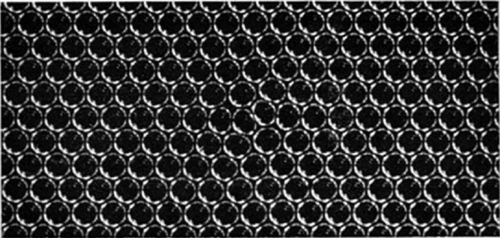
\includegraphics[width=0.7\linewidth]{fyz_fig763.jpg}
      \caption{
               (\cite[s.~707]{Feynman02})}
      \label{fyz_fig763}
    \end{figure}

    \begin{figure}[ht!] %\ref{fyz_fig764}
      \centering
      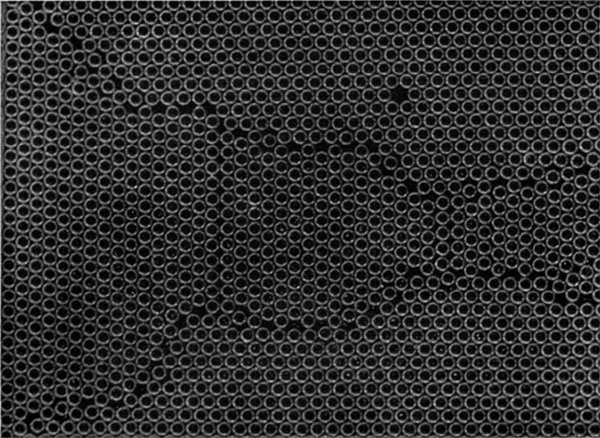
\includegraphics[width=0.7\linewidth]{fyz_fig764.jpg}
      \caption{
               (\cite[s.~707]{Feynman02})}
      \label{fyz_fig764}
    \end{figure}

    \begin{figure}[ht!] %\ref{fyz_fig765}
      \centering
      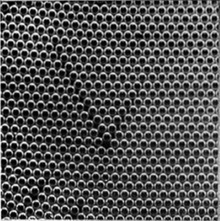
\includegraphics[width=0.7\linewidth]{fyz_fig765.jpg}
      \caption{
               (\cite[s.~707]{Feynman02})}
      \label{fyz_fig765}
    \end{figure}
    
    \begin{figure}[ht!] %\ref{fyz_fig766}
      \centering
      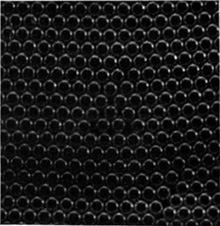
\includegraphics[width=0.7\linewidth]{fyz_fig766.jpg}
      \caption{
               (\cite[s.~707]{Feynman02})}
      \label{fyz_fig766}
    \end{figure}

    \begin{figure}[ht!] %\ref{fyz_fig767}
      \centering
      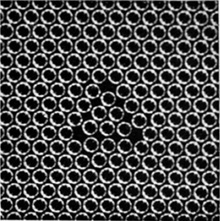
\includegraphics[width=0.7\linewidth]{fyz_fig767.jpg}
      \caption{
               (\cite[s.~707]{Feynman02})}
      \label{fyz_fig767}
    \end{figure}

    \begin{figure}[ht!] %\ref{fyz_fig768}
      \centering
      \includegraphics[width=0.7\linewidth]{fyz_fig768.jpg}
      \caption{
               (\cite[s.~707]{Feynman02})}
      \label{fyz_fig768}
    \end{figure}

    \begin{figure}[ht!] %\ref{fyz_fig769}
      \centering
      \includegraphics[width=0.7\linewidth]{fyz_fig769.jpg}
      \caption{
               (\cite[s.~707]{Feynman02})}
      \label{fyz_fig769}
    \end{figure}

    \begin{figure}[ht!] %\ref{fyz_fig770}
      \centering
      \includegraphics[width=0.7\linewidth]{fyz_fig770.jpg}
      \caption{
               (\cite[s.~707]{Feynman02})}
      \label{fyz_fig770}
    \end{figure}

    \begin{figure}[ht!] %\ref{fyz_fig771}
      \centering
      \includegraphics[width=0.7\linewidth]{fyz_fig771.jpg}
      \caption{
               (\cite[s.~707]{Feynman02})}
      \label{fyz_fig771}
    \end{figure}

    \begin{figure}[ht!] %\ref{fyz_fig772}
      \centering
      \includegraphics[width=0.7\linewidth]{fyz_fig772.jpg}
      \caption{
               (\cite[s.~707]{Feynman02})}
      \label{fyz_fig772}
    \end{figure}

    \begin{figure}[ht!] %\ref{fyz_fig773}
      \centering
      \includegraphics[width=0.7\linewidth]{fyz_fig773.jpg}
      \caption{
               (\cite[s.~707]{Feynman02})}
      \label{fyz_fig773}
    \end{figure}

    \begin{figure}[ht!] %\ref{fyz_fig774}
      \centering
      \includegraphics[width=0.7\linewidth]{fyz_fig774.jpg}
      \caption{
               (\cite[s.~707]{Feynman02})}
      \label{fyz_fig774}
    \end{figure}

    \begin{figure}[ht!] %\ref{fyz_fig775}
      \centering
      \includegraphics[width=0.7\linewidth]{fyz_fig775.jpg}
      \caption{
               (\cite[s.~707]{Feynman02})}
      \label{fyz_fig775}
    \end{figure}

    \begin{figure}[ht!] %\ref{fyz_fig776}
      \centering
      \includegraphics[width=0.7\linewidth]{fyz_fig776.jpg}
      \caption{
               (\cite[s.~707]{Feynman02})}
      \label{fyz_fig776}
    \end{figure}

    \begin{figure}[ht!] %\ref{fyz_fig777}
      \centering
      \includegraphics[width=0.7\linewidth]{fyz_fig777.jpg}
      \caption{
               (\cite[s.~707]{Feynman02})}
      \label{fyz_fig777}
    \end{figure}

    \begin{figure}[ht!] %\ref{fyz_fig778}
      \centering
      \includegraphics[width=0.7\linewidth]{fyz_fig778.jpg}
      \caption{
               (\cite[s.~707]{Feynman02})}
      \label{fyz_fig778}
    \end{figure}

    \begin{figure}[ht!] %\ref{fyz_fig779}
      \centering
      \includegraphics[width=0.7\linewidth]{fyz_fig779.jpg}
      \caption{
               (\cite[s.~707]{Feynman02})}
      \label{fyz_fig779}
    \end{figure}

    \begin{figure}[ht!] %\ref{fyz_fig780}
      \centering
      \includegraphics[width=0.7\linewidth]{fyz_fig780.jpg}
      \caption{
               (\cite[s.~707]{Feynman02})}
      \label{fyz_fig780}
    \end{figure}

    \begin{figure}[ht!] %\ref{fyz_fig781}
      \centering
      \includegraphics[width=0.7\linewidth]{fyz_fig781.jpg}
      \caption{
               (\cite[s.~707]{Feynman02})}
      \label{fyz_fig781}
    \end{figure}

    \begin{figure}[ht!] %\ref{fyz_fig782}
      \centering
      \includegraphics[width=0.7\linewidth]{fyz_fig782.jpg}
      \caption{
               (\cite[s.~707]{Feynman02})}
      \label{fyz_fig782}
    \end{figure}

    \begin{figure}[ht!] %\ref{fyz_fig783}
      \centering
      \includegraphics[width=0.7\linewidth]{fyz_fig783.jpg}
      \caption{
               (\cite[s.~707]{Feynman02})}
      \label{fyz_fig783}
    \end{figure}

    \begin{figure}[ht!] %\ref{fyz_fig784}
      \centering
      \includegraphics[width=0.7\linewidth]{fyz_fig784.jpg}
      \caption{
               (\cite[s.~707]{Feynman02})}
      \label{fyz_fig784}
    \end{figure}

    \begin{figure}[ht!] %\ref{fyz_fig785}
      \centering
      \includegraphics[width=0.7\linewidth]{fyz_fig785.jpg}
      \caption{
               (\cite[s.~707]{Feynman02})}
      \label{fyz_fig785}
    \end{figure}

    \begin{figure}[ht!] %\ref{fyz_fig786}
      \centering
      \includegraphics[width=0.7\linewidth]{fyz_fig786.jpg}
      \caption{
               (\cite[s.~707]{Feynman02})}
      \label{fyz_fig786}
    \end{figure}

    \begin{figure}[ht!] %\ref{fyz_fig787}
      \centering
      \includegraphics[width=0.7\linewidth]{fyz_fig787.jpg}
      \caption{
               (\cite[s.~707]{Feynman02})}
      \label{fyz_fig787}
    \end{figure}


  \section{Příklady a cvičení}\label{fyz:IIchapXXXsecX}


%} %tikzset
%---------------------------------------------------------------------------------------------------
\printbibliography[title={Seznam literatury},heading=subbibliography]
\addcontentsline{toc}{section}{Seznam literatury}